\pagenumbering{arabic}
\documentclass{beamer}
\newlength{\wideitemsep}
\setlength{\wideitemsep}{\itemsep}
\addtolength{\wideitemsep}{1pt}
\let\olditem\item
\renewcommand{\item}{\setlength{\itemsep}{\wideitemsep}\olditem}
% By  using hyperref={pdfpagelabels=false} you get rid off:
% Package hyperref Warning: Option `pdfpagelabels' is turned off
% (hyperref)                because \thepage is undefined.
% Hyperref stopped early
%
\usetheme{Singapore}
%\setbeamertemplate{footline}[frame number]

\usepackage{color}
\usepackage{algorithm, algorithmic}
\usepackage{ mathrsfs }
\usepackage{ dsfont }
\usepackage{lmodern}
\usepackage{array}
\usepackage{bbm}
\usepackage{amsmath}
\usepackage{amssymb}
\usepackage[mathscr]{eucal}
\usepackage{graphicx}
\usepackage{mathrsfs}
\usepackage{psfrag}
\usepackage{color}
\usepackage{here}
\usepackage{media9}
\usepackage{hyperref}
\usepackage{wasysym}


% Using lmondern and you get rid off this:
% LaTeX Font Warning: Font shape `OT1/cmss/m/n' in size <4> not available
% (Font)              size <5> substituted on input line 22.
% LaTeX Font Warning: Size substitutions with differences
% (Font)              up to 1.0pt have occurred.
%

% If \titel{$B!D(B} \author{$B!D(B} come after \begin{document}
% you get the following warnig:
% Package hyperref Warning: Option `pdfauthor' has already been used,
% (hyperref) ...
% So it is here before \begin{document}


\title{Near-optimal Reinforcement Learning in Factored MDPs}
\author{Ian Osband \and Benjamin Van Roy}
\institute{Mangement Science and Engineering \\
Stanford University \\
iosband@stanford.edu}
\date{\today}
% additional usepackage{beamerthemeshadow} is used
% and  \beamersetuncovermixins{\opaqueness<1>{25}}{\opaqueness<2->{15}}
% with this the elements which were coming soon were only hinted
%
%\usepackage{beamerthemeshadow}
%\beamersetuncovermixins{\opaqueness<1>{25}}{\opaqueness<2->{15}}

%\theoremstyle{break}
\newtheorem{mydef}{Definition}
\newtheorem{prop}{Proposition}
\newtheorem{claim}{Claim}

%-------------------- Macros -------------------------------------------------------------------------------------------------------------------------------------
% Setting up macro shortcuts
\newcommand{\Exp}{\mathds{E}}
\newcommand{\Expk}{\mathds{E}_{k}}
\newcommand{\Prob}{\mathds{P}}
\newcommand{\Real}{\mathds{R}}
\newcommand{\Nat}{\mathbb{N}}
\newcommand{\Ind}{\mathds{1}}

\newcommand{\Xc}{\mathcal{X}}
\newcommand{\Yc}{\mathcal{Y}}
\newcommand{\Pc}{\mathcal{P}}
\newcommand{\Qc}{\mathcal{Q}}
\newcommand{\Fc}{\mathcal{F}}
\newcommand{\Gc}{\mathcal{G}}
\newcommand{\Rc}{\mathcal{R}}
\newcommand{\Sc}{\mathcal{S}}
\newcommand{\Ac}{\mathcal{A}}
\newcommand{\Mc}{\mathcal{M}}
\newcommand{\Tc}{\mathcal{T}}
\newcommand{\Dep}{ \Delta^H,\Delta^F,\mathcal{F},\epsilon }

\newcommand{\conf}{\mathcal{F}^d_t}

\newcommand{\vect}[1]{\boldsymbol{#1}}
\newcommand{\opt}{M^*}
\newcommand{\sampled}{{M_k}}
\newcommand{\Pstar}{P^{*}(\cdot \mid s_t, a_t)}
\newcommand{\Pk}{P_{k}(\cdot \mid s_t, a_t)}
\newcommand{\Pdiff}{(P_{k}-P^{*})(\cdot \mid s_t, a_t)}
\newcommand{\Rdiff}{(r_k-r^{*})(s_t, a_t)}
\newcommand{\optPol}{\mu^{*}}
\newcommand{\sampledPol}{\mu_{k}}
\newcommand{\bellmanSampled}{\mathcal{T}_{\mu_{k}(\cdot,i)}^{k}}
\newcommand{\bellmanTrue}{\mathcal{T}_{\mu_{k}(\cdot,i)}^{*}}
\newcommand{\bellmanSampledA}{\mathcal{T}_{\mu_{k}(\cdot,1)}^{k}}
\newcommand{\bellmanTrueA}{\mathcal{T}_{\mu_{k}(\cdot,1)}^{*}}
\newcommand{\vSampled}{V_{\mu_k, 1}^{k}}
\newcommand{\vSampledi}{V_{\mu_k, i}^{k}}
\newcommand{\vTrue}{V_{\tau, \mu_k}^{*}}

%-----------------------------------------------------------------------------------------------------------------------------------------------------------------------






%-------------- Start of the actual presentation -------------------------------------------------------------------------------------------------------------------
\begin{document}

\maketitle

\begin{frame}
\frametitle{Table of contents}
\tableofcontents
\end{frame}

%---------------------------------------------------------------------------------------------------
% Problem Specification - overview and big picture
\section{Reinforcement Learning}

% Slide
\begin{frame}
\frametitle{Reinforcement Learning}

\begin{itemize}
	\item We imagine an agent taking actions within an environment.
	\item Actions serve two purposes:
	\begin{itemize}
		\item Instantaneous loss/reward to the agent.
		\item Influence the state of the environement.
	\end{itemize}
	\item The agent wants to maximize cumulative reward through time.
	\item How can an agent learn to take ``good" actions?
	\pause
	\vspace{0.5in}
	\item Multi-armed bandit with added state transitions.
	\item Statistical estimation + optimal control.
	\pause
	\item \dots this could get hard!
\end{itemize}
\end{frame}

% Slide
\begin{frame}
\frametitle{Mouse in a maze}
\begin{figure}
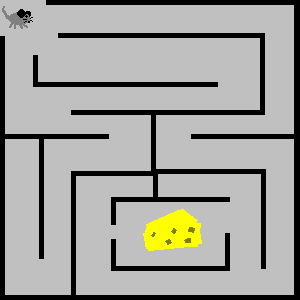
\includegraphics[width=0.55\textwidth]{./media/mazeCheese}
\end{figure}
\centering
What's the best way to the cheese?
\end{frame}

% Slide
\begin{frame}
\frametitle{Self-driving car}
\begin{figure}
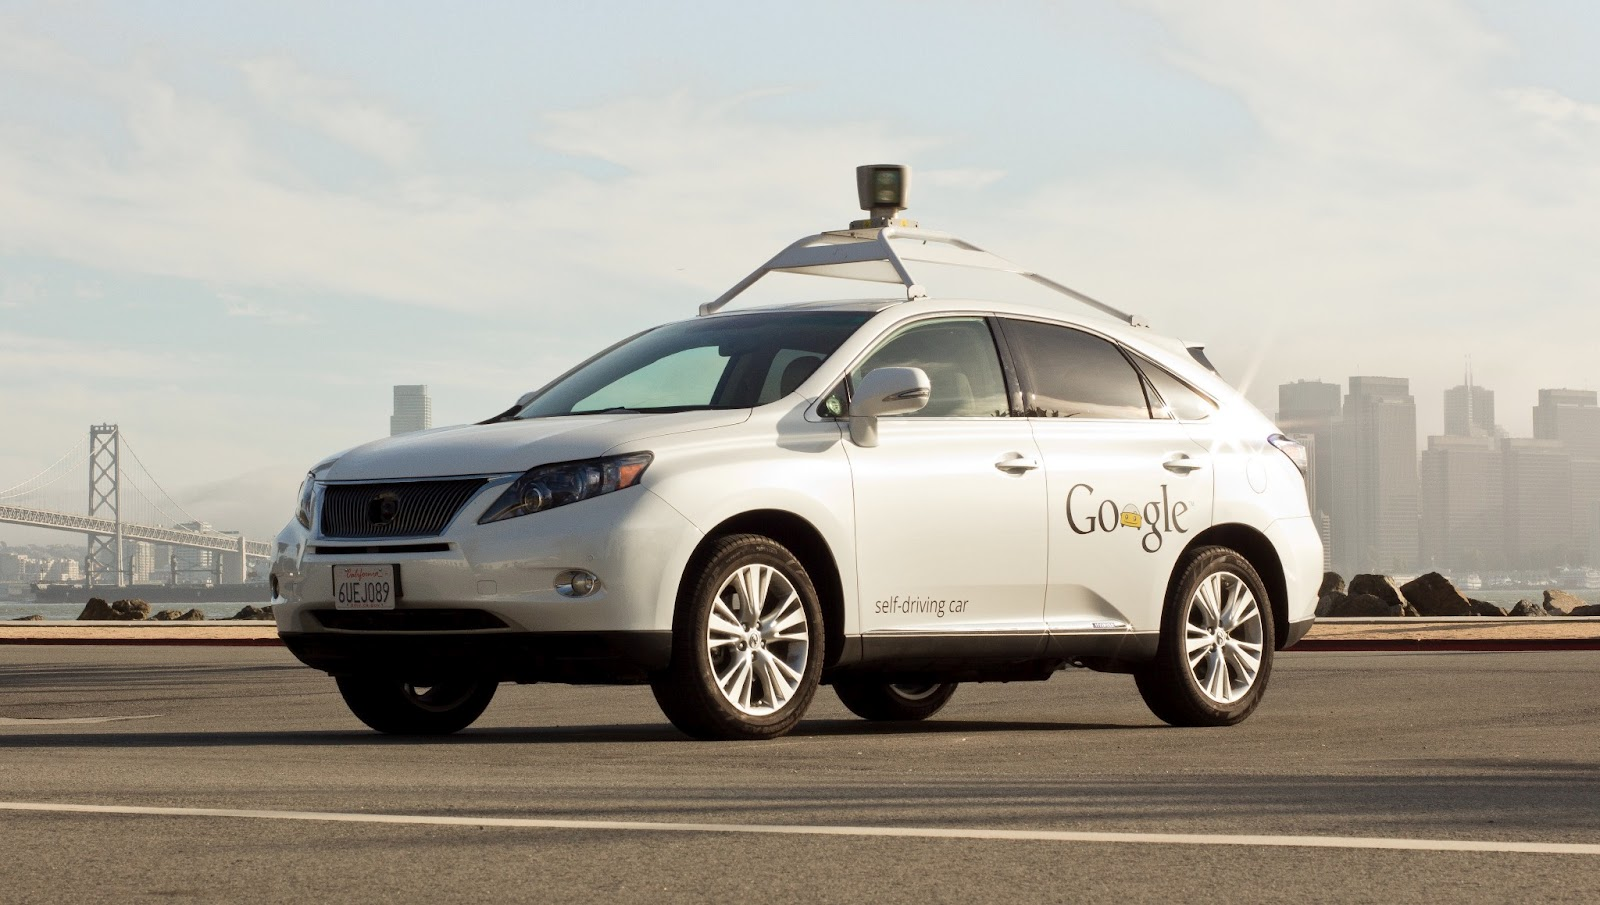
\includegraphics[width=0.85\textwidth]{./media/selfCar}
\end{figure}
\centering
Drive me from A to B\pause\dots also don't kill anyone.
\end{frame}

% Slide
\begin{frame}
\frametitle{Markov decision process (MDP)}

\begin{itemize}
	\item Model decision making in a stochastic environment.
	\item At time $t$ the agent in state $s_t \in \Sc$ chooses action $a_t \in \Ac$.
	\item Reward $r_t \sim R(s_t,a_t)$ and transition to $s_{t+1} \sim P(\cdot | s_t,a_t)$.
	\item Given $R,P$ there is some optimal policy $\pi^*:s_t \rightarrow a^*_t$.
	\item Generally this is computed via Dynamic Programming.
	\pause
	\vspace{8mm}
	\item In reinforcement learning, the agent is unsure of $P,R$.
	\item The learning algorithm will pick $\pi^L_t : s_t \rightarrow a_t^L$.
	\item We would like to get average reward $\rho(\pi^L)$ close to $\rho(\pi^*)$.
\end{itemize}
\end{frame}


%---------------------------------------------------------------------------------------------------
% Efficienct reinforcement learning
\section{Efficienct RL}
% Slide
\begin{frame}
\frametitle{Efficient reinforcement learning}

\begin{itemize}
	\item Will we learn the best policy?
	$$ \rho(\pi^L_t) \rightarrow \rho(\pi^*)$$ \pause
	\item How long do we have to wait to do well? (Sample complexity)
	$$ \forall t > T({\rm MDP},\pi^L) \ \ \ \rho(\pi^L_t) \ge \rho(\pi^*) -\epsilon $$ \pause
	\item How badly do we do while we're learning? (Regret)
	$$ {\rm Regret}(T,\pi^L) = \sum_{t=1}^T r^*_t - r_t \le f({\rm MDP},T,\pi^L) $$
\end{itemize}
\end{frame}

% Slide
\begin{frame}
\frametitle{Reward and transition functions}
We will specialize our analysis two important function classes:

\begin{mydef}[Reward functions $\in \Pc^{C,\sigma}_{\Sc \times \Ac,\Real} $]
$\Pc^{C,\sigma}_{\Xc,\Real}$ is the set of functions from $\Xc$ to $\sigma$-sub gaussian measures over $(\Real,\mathcal{B}(\Real) )$ with mean in $[0,C]$.
\end{mydef}

\begin{mydef}[Transition functions $\in \Pc_{\Sc \times \Ac,\Sc}$]
$\Pc_{\Xc,\Yc}$ is the set of functions mapping elements of a finite set $\Xc$ to probability mass functions over a finite set $\Yc$.
\end{mydef}
\end{frame}

% Slide
\begin{frame}
\frametitle{Regret bounds}
\begin{itemize}
	\item Greedy algorithms may never learn $\rho(\pi^L_t) \nrightarrow \rho(\phi^*)$.
	\item Na\"{i}ve exploration leads to regret exponential in $|\Sc|, |\Ac|$.
	\item Efficient algorithms must guide their exploration:
	\begin{itemize} \pause
		\item ``Optimism in the face of uncertainty'' (OFU).
		\item ``Posterior sampling'' (PS)
	\end{itemize}
	\pause \vspace{3mm}
	\item Efficent algorithms with Regret $\tilde{O}(|\Sc| \sqrt{|\Ac|T})$.
	\item Lower bound on Regret $\Omega(\sqrt{|\Sc| |\Ac| T})$.
	\item But in many cases of interest $\Sc, \Ac$ are huge... \pause \frownie
\end{itemize}
\end{frame}

%---------------------------------------------------------------------------------------------------
% Factored MDPS
\section{Factored MDPs}
\begin{frame}
\frametitle{Factored MDPs}
\centering
\begin{figure}
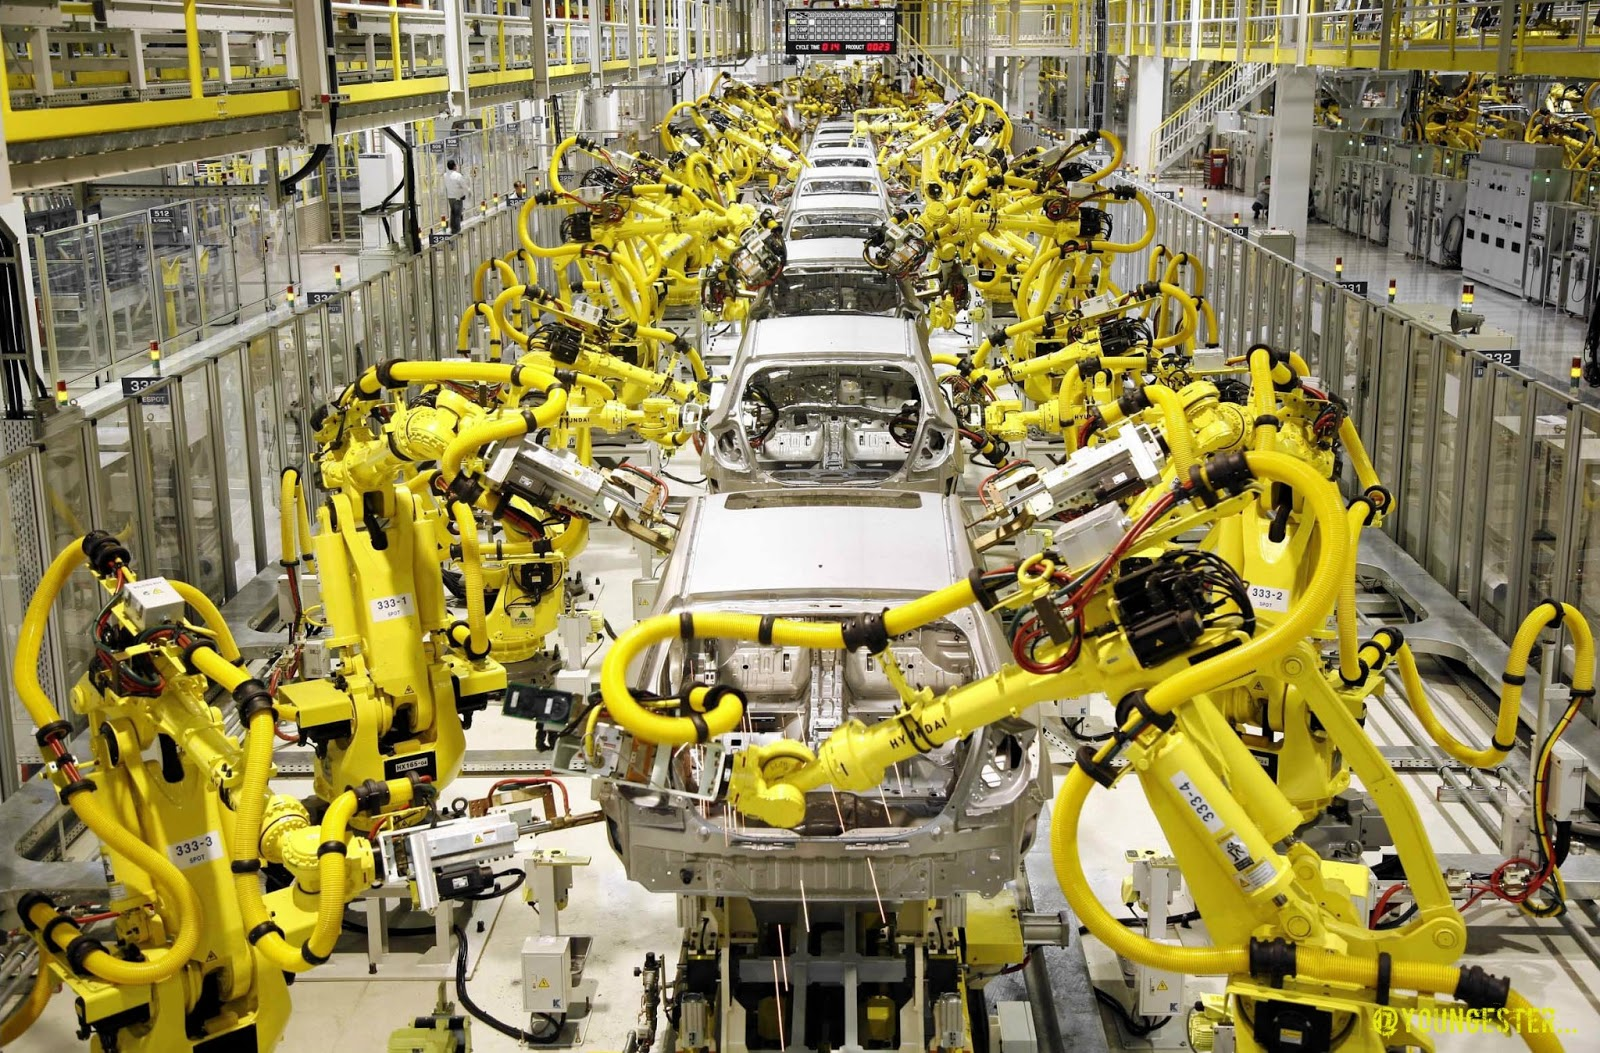
\includegraphics[width=0.75\textwidth]{./media/productionLine}
\end{figure}
Each transition only depends \underline{directly} on a subset of the MDP.
\end{frame}


% Slide
\begin{frame}
\frametitle{Factored MDPs}
Let $\Sc \times \Ac = \Xc = \Xc_1 \times .. \times \Xc_n$, $Z \subseteq [n]$ and
$ \Xc[Z] := \bigotimes\limits_{i \in Z} \Xc_i $

\begin{mydef}[ Factored reward functions $R \in \Rc \subseteq \Pc^{C,\sigma}_{\Xc,\Real} $]
$\Rc$ is factored over $\Xc = \Xc_1 \times .. \times \Xc_n $ with scopes $Z_1, .. Z_l$ $\iff$,
for all $R \in \Rc, x \in \Xc$ there exist,
\begin{center}
$ \Exp [ R(x) ] = \sum_{i=1}^l \Exp\big[ R_i(x[Z_i]) \big] $
\end{center}
with each $r_i \sim R_i(x[Z_i])$ and individually observed.
\end{mydef}


\begin{mydef}[ Factored transition functions $P \in \Pc \subseteq \Pc_{\Xc,\Sc}$ ]
$\Pc$ is factored over $\Xc = \Xc_1 \times .. \times \Xc_n$ and $\Sc = \Sc_1 \times .. \times \Sc_m$ with scopes  $Z_1, .. Z_m$ $\iff$,
for all $P \in \Pc, x \in \Xc, s \in \Sc$ there exist,
$$ P(s | x) = \prod_{i=1}^m P_i \left( s[i] \ \bigg\vert \ x[Z_i] \right) $$
\end{mydef}
\end{frame}

% Slide
\begin{frame}
\frametitle{Factored MDPs}

\begin{itemize}
	\item Agent knows $\Gc  = \big( \{ \Sc_i \}_{i=1}^m ; \  \{ \Xc_i \}_{i=1}^n ; \   \{ Z^R_i \}_{i=1}^l;\  \{ Z^P_i \}_{i=1}^m \big)$.
	\item Must learn $\big( \{R_i \}_{i=1}^l;\  \{ P_i \}_{i=1}^m \big) $ from experience.
	\item Algorithms ignoring $\Gc$ lead to exponential regret bounds.
	\item $|\Sc| = \prod_{i=1}^m|\Sc_i| = |\Sc_1|^m, \ \ \ |\Sc| |\Ac| = \prod_{i=1}^n|\Xc_i| = |\Xc_1|^n$
	\vspace{1cm}
	\pause
	%\item Let $|\Sc_i| = |\Xc_i| = K$, $|Z^R_i| = |Z^P_i| = \zeta$ for $i=1,..,m$
	% \item Write $J = K^\zeta$ for $\lambda = m / \zeta \gg 1$.
	% \item $|\Sc| \sqrt{|\Ac|T} \ge \sqrt{J^\lambda K^m T}$ which is an exponential dependence!
	\item Efficient complexity bounds exist polynomial in $|\Xc_i|,|\Sc_i|$
	\item No such results for regret\dots \pause until now.
\end{itemize}
\end{frame}


%---------------------------------------------------------------------------------------------------
% Main
\section{Main results}

% Slide
\begin{frame}
\frametitle{Posterior Sampling for Reinforcement Learning}

\begin{algorithm}[H]
\label{alg: PSRL}

\begin{algorithmic}[1]
	\STATE \textbf{Input: }Prior $\phi$ encoding $\Gc$, $t=1$
	\FOR{episodes $k=1,2,..$}
		\STATE{sample $M_k \sim \phi(\cdot | H_{t})$}
		\STATE{compute $\mu_k = \Gamma(M_k,\sqrt{\tau / k})$}  \textcolor{magenta}{$\leftarrow$(ADP planner)}

		\FOR{timesteps $j=1,..,\tau$}
			\STATE{sample and apply $a_t = \mu_k(s_t,j)$}
			\STATE{observe $r^1_t,..,r^l_t$ and $s^1_{t+1},..,s^m_{t+1}$}
			\STATE{$t = t+1$}
		\ENDFOR

	\ENDFOR
\end{algorithmic}
\end{algorithm}
\end{frame}

% Slide
\begin{frame}
\frametitle{UCRL-Factored}

\footnotesize
\begin{algorithm}[H]
\label{alg: UCRL-Factored}
\footnotesize
\begin{algorithmic}[1]
	\STATE \textbf{Input: }Graph structure $\Gc$, confidence $\delta$, $t=1$
	\FOR{episodes $k=1,2,..$}
		\STATE{$d_t^{R_i} = 4 \sigma^2 \log\left(4 l | \Xc[Z^R_i] | k / \delta\right)$ for $i=1,..,l$}
		\STATE{$d_t^{P_j} = 4 | \Sc_j | \log\left(4 m | \Xc[Z^P_j] | k  / \delta\right)$ for $j=1,..,m$}
		\STATE{ $\Mc_k = \{M \ | \Gc, \overline{R}_i \in \Rc^i_t(d_t^{R_i}), P_j \in \Pc^j_t(d_t^{P_j}) \ \forall i,j \}$} \textcolor{magenta}{$\leftarrow$(Confidence sets)}
		\STATE{compute $\mu_k = \tilde{\Gamma}(\Mc_k,\sqrt{\tau / k})$} $\leftarrow$ \textcolor{magenta}{$\leftarrow$(ADP planner)}

		\FOR{timesteps $u=1,..,\tau$}
			\STATE{sample and apply $a_t = \mu_k(s_t,u)$}
			\STATE{observe $r^1_t,..,r^l_t$ and $s^1_{t+1},..,s^m_{t+1}$}
			\STATE{$t = t+1$}
		\ENDFOR

	\ENDFOR
\end{algorithmic}

\end{algorithm}
\end{frame}

% Slide
\begin{frame}
\frametitle{Main results}
\begin{theorem}[Expected regret for PSRL in factored MDPs]
\label{thm: reg PSRL}
If the prior $\phi$ is the distribution of $M^*$ and $\Psi$ is the span of the optimal value function:
\footnotesize
\begin{equation}
	\Exp \left[\mathrm{Regret}(T, \pi^{\rm PS}_{\tau}, M^*) \right] =
	\tilde{O}\left( \sigma \sum_{i=1}^{d_1} \sqrt{ | \Xc[Z^R_i] |T} + \Exp[ \Psi ] \sum_{j=1}^{d_2} \sqrt{|\Xc[Z^P_j]| |\Sc_j| T} \right)
\end{equation}
\end{theorem}


\begin{theorem}[High probability regret for UCRL-Factored]
\label{thm: reg UCRL-Factored}
If $D$ is the diameter of $M^*$, then for any $M^*$ can bound the regret of UCRL-Factored:
\footnotesize
\begin{equation}
	\mathrm{Regret}(T, \pi^{\rm UC}_{\tau}, M^*) =
	\tilde{O}\left( \sigma \sum_{i=1}^{d_1} \sqrt{ | \Xc[Z^R_i] |T} + C D \sum_{j=1}^{d_2} \sqrt{|\Xc[Z^P_j]| |\Sc_j| T} \right)
\end{equation}
\normalsize
with probability at least $1-\delta$
\end{theorem}
\end{frame}

% Slide
\begin{frame}
\frametitle{Clean bounds in the symmetric case}
Let $\Qc$ be shorthand for the structure $\Gc$ such that $l+1=m$, $C=\sigma=1$, $| \Sc_i | = |\Xc_i | = K$ and $|Z^R_i| = |Z^P_i | = \zeta$ for all suitable $i$ and write $J = K^\zeta$.
In this case $\Psi, D \le \tau$ trivially.
\vspace{2mm}

\begin{corollary}[Clean bounds for PSRL]
\label{cor: reg PSRL}
\begin{equation}
	\Exp \left[\mathrm{Regret}(T, \pi^{\rm PS}_{\tau}, M^*) \right]
	\le 15m \tau \sqrt{J K T \log(2mJ T)}
\end{equation}
\end{corollary}

\begin{corollary}[Clean bounds for UCRL-Factored]
\label{cor: reg UCRL-Factored}
\begin{equation}
	\mathrm{Regret}(T, \pi^{\rm UC}_{\tau}, M^*) \le  15m \tau \sqrt{J K T \log(12mJT / \delta)}
\end{equation}
with probability at least $1-\delta$.
\end{corollary}
\end{frame}

% Slide
\begin{frame}
\frametitle{Clean bounds in the symmetric case}
Let $\Qc$ be shorthand for the structure $\Gc$ such that $l+1=m$, $C=\sigma=1$, $| \Sc_i | = |\Xc_i | = K$ and $|Z^R_i| = |Z^P_i | = \zeta$ for all suitable $i$ and write $J = K^\zeta$.
In this case $\Psi, D \le \tau$ trivially.
\vspace{7mm}

The key point is that we go from $\Gc$-agnostic
$$ \tilde{O}(|\Sc| \sqrt{|\Ac|T}) = \tilde{O}(\sqrt{J^{m/\zeta} K^{m} T})$$
to the new bounds
$$ \tilde{O}(\sum_{j=1}^{m}\sqrt{|\Xc[Z^P_j]||\Sc_j|T}) = \tilde{O}(m \sqrt{J K T})$$
which can be exponentially tighter.
\end{frame}

% Slide
\begin{frame}
\frametitle{Analysis outline}
\small
We consider $Regret(T) = \sum_{k=1}^m \Delta_k$, regret within each episode.
\begin{equation}
	\Delta_k =  V^*_{*,1}(s) - V^*_{k,1}(s) = \bigg( V^k_{k,1}(s) - V^*_{k,1}(s) \bigg) + \bigg(V^*_{*,1}(s) - V^k_{k,1}(s) \bigg)
\end{equation}
Where $V^M_{\mu,1}(s)$ is the value of empolying policy $\mu$ on MDP $M$ for one episode.
We write $*,k$ as shorthand for the optimal and algorithmic MDPs at each stage.
\small
\begin{equation}
	\left(V^k_{k,1} - V^*_{k,1} \right) (s_{t_k+1}) = \sum_{i=1}^\tau \left( \Tc^k_{k,i} - \Tc^*_{k,i} \right) V^k_{k,i+1}(s_{t_k+i}) + \sum_{i=1}^\tau d_{t_k+1}.
\end{equation}
Where $d_t$ is a bounded martingale difference and the first term $A$:
\begin{equation}
\label{eq: err sums}
	A \le \sum_{i=1}^\tau |\overline{R}^k(x_{k,i}) - \overline{R}^*(x_{k,i}) | +
	\frac{1}{2} \Psi_k \|P^k(\cdot|x_{k,i}) - P^*(\cdot|x_{k,i}) \|_1
\end{equation}
\end{frame}


% Slide
\begin{frame}
\frametitle{Key lemma}
\begin{lemma}[Bounding factored deviations]
\label{lem: factor bound} \hspace{0.000000001mm} \newline
Let the transition function class $\Pc \subseteq \Pc_{\Xc,\Sc}$ be factored over $\Xc = \Xc_1 \times .. \times \Xc_n$ and $\Sc = \Sc_1 \times .. \times \Sc_m$ with scopes  $Z_1, .. Z_m$.
Then, for any $P,\tilde{P} \in \Pc$ we may bound their L1 distance by the sum of the differences of their factorizations:
$$ \| P(x) - \tilde{P}(x) \|_1 \le \sum_{i=1}^m \|P_i(x[Z_i]) - \tilde{P}_i(x[Z_i]) \|_1 $$
\end{lemma}

Using Azuma-Hoeffding with a union bound we can bound the Bellman error in terms of a concentration which depends on $|\Xc[Z_i^P]|$ as opposed to $|\Xc|$.
From the previous slide this gives us bounds on regret.
\end{frame}

% Slide
\begin{frame}
\frametitle{References}
\centering
Please see arXiv for a full version of the paper.
\vspace{1cm}

\pause
Thanks!
\end{frame}

\end{document}
